
\documentclass[12pt]{amsart}
\usepackage{subfig}
\usepackage{float}
\usepackage{graphicx}
\usepackage{geometry} % see geometry.pdf on how to lay out the page. There's lots.
\geometry{a4paper} % or letter or a5paper or ... etc
% \geometry{landscape} % rotated page geometry

% See the ``Article customise'' template for come common customisations

\title{Computer Vision}
\author{Anouk Visser and R\'emi de Zoeten}
\date{} % delete this line to display the current date

%%% BEGIN DOCUMENT
\begin{document}

\maketitle
%\tableofcontents

\section{Assignment 1}
\subsection{ICP}
There are different ways to improve the efficiency and the accuracy of ICP. Some of these techniques are discussed in ``Efficient variants of the ICP algorithm.''. In this assignment, students should also analyze various aspects such as accuracy, speed, stability and tolerance to noise by changing the point selection technique. Using all the points, uniform sub-sampling, random sub-sampling in each iteration and sub-sampling more from informative regions can be used as the point selection technique. Students are expected to implement these variants and report their findings in the final report.\\

We implemented the ICP algorithm and three different sampling methods. We implemented the uniform sampling method by sampling points from the data at a uniform interval. We implemented the random sampling method using matlab's built in \textit{datasample} method. Furthermore, we implemented a `Nearest neighbor' sampling method that is designed to sample more at the informative edges of the structure than at the less informative center. This is done by finding the min and max $x, y$ and $z$ values and sampling uniformly random between e.g. the $x_{min}$ and $x_{max}$ interval. Once the random values $x_r, y_r, z_r$ are selected, a k-d tree is used to find the nearest point in the data. This method works best for data that represents a convex structure, and we performed measurements to discover if this method performs well for sampling our data.
Figure \ref{comp} shows our results for the comparison of different sampling methods. For this experiment we used our icp method to align images 20 and 25 from the dataset. The icp algorithm used 7 iterations. The first 6 sampled $10\%$ of the points, and in the last iteration all points were used. We plotter the root mean squared error (RMS) for each method at each iteration. We also provided the runtime that was needed to perform all 7 icp iterations, sampling included.

\begin{figure}[H]
\center
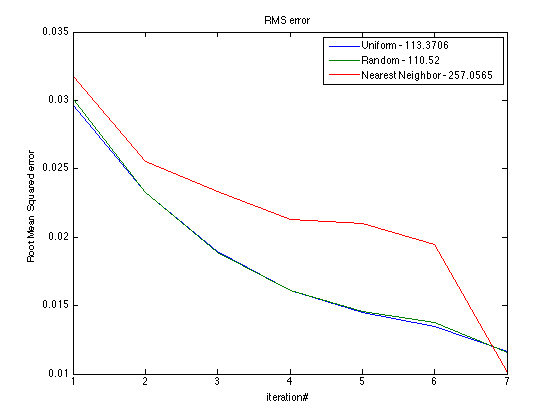
\includegraphics[scale=0.5]{images/comparison.png}
\caption{comp.}
\label{comp}
\end{figure}

As can be seen in figure \ref{comp}, the random and uniform sampling methods perform very similar in time and RMS over all iterations. The Nearest Neighbor sampling method seems to have a higher RMS at early iterations, but suddenly drops at the last iteration where no subsampling is used. This means that although the RMS is higher using the Nearest Neighbor sampling method, the learned transformations are more accurate, leading to a lower final RMS. Because the Nearest Neighbor sampler needs to search the kd-tree for each sample that is taken from the data, the time that is used by this method is ~2.5 times longer. We think that if time is a consideration then in our implementation the random sampling method should be used.


\subsection{Merging scenes}
Estimate the camera poses using each two consecutive frames of given data. Using the estimated camera poses, merge the point-clouds of all the scenes into one point-cloud and visualize the result. 
\\\\
\textbf{Does the merging produce sufficient result? Discuss why.}
\\\\
\textbf{Now, estimate the camera pose and merge the results using every 2nd, 4th, and 10th frames. Does the camera pose estimation change?}
\\\\
Iteratively merge and estimate the camera poses for the consecutive frames (point-clouds). Supposed there are N frames (frame1, frame2 ,. . ., frameN). First, estimate the camera pose of frame2 (target) from frame1(base). Next, merge frame1 and frame2 into frame1,2. Then, estimate the camera pose of frame3(target) from frame1,2(base) and use it to merge frame1,2 and frame3 into frame1,2,3 and so on until reaching the final frame (frameN ).\\\\ \textbf{Do the estimated camera poses change in comparison with the previous estimates (Section 2.1)? Does this estimation produce better results?}
\subsection{Questions}
\textbf{What are the drawbacks of the ICP algorithm?}\\\\
\textbf{How do you think the ICP algorithm can be improved, beside the techniques mentioned in ``Efficient variants of the ICP algorithm.'', in terms of efficiency and accuracy?}

One disadvantage of the ICP algorithm is that the initial alignment can not be too far of. This is because ICP is a form of hill-climbing where any one optimum might not necessarily be the global optimum. This problem might not be an issue in all domains. 
One method to improve the ICP performance is to improve the data sampling method. What might help in some cases is to sample from the contours of the structure. Another might be to on-the-fly find out what kind of sampling works best for the specific task.

\section{Assignment 2}
\subsection{Fundamental Matrix Estimation}
To estimate the fundamental matrix $F$ we implemented the eight-point algorithm, the normalized eight-point algorithm and the normalized eight-point algorithm with RANSAC. Before we can estimate the fundamental matrix we need a set of corresponding points across two images. Therefore we first detect interest points in each image and extract their descriptors in order to match the interest points. We discard all matches that are in the background using the method described in section \ref{background}. The matches can then be used to estimate the fundamental matrix. \\\\
To check the correctness of the fundamental matrix estimation algorithms we verified that the fundamental matrix was singular ($\textit{det}(M) = 0$ for singular matrix $M$ ). We present our analysis of the estimation of the fundamental matrix for the first and second teddy-bear images in table \ref{fund}.
\begin{table}
\center
    \begin{tabular}{l|l|l|l}
    ~                  & ep & nep & nepR \\ \hline
    F                  
    & $\bigl(\begin{smallmatrix}0.0000&0.0000&-0.0019\\ 0.0000&0.0000&-0.0009\\-0.0029&-0.0024&1.0000\end{smallmatrix} \bigr)$ 
    & $\bigl(\begin{smallmatrix}0.0000&0.0000&-0.0112\\ -0.0001&0.0000&-0.0001\\0.0222&-0.0012&-1.4995\end{smallmatrix} \bigr)$                      
    & $\bigl(\begin{smallmatrix}0.0000&0.0002&-0.0438\\ -0.0002&0.0000&0.0575\\0.0562&-0.0470&-3.2704\end{smallmatrix} \bigr)$                                  \\ \hline
    det(F)             & 5.3517e-28  & 1.5718e-24             & -1.3839e-22                        \\ \hline
    elapsed time (sec) & 0.000807    & 0.151748               & 0.833404                           \\
    \end{tabular}
    \caption{Fundamental matrix $F$, $\textit{det}(F)$ and the elapsed time in seconds to calculate $F$ for the eight-point algorithm (ep), normalized eight-point algorithm (nep) and the normalized eight-point algorithm with RANSAC (nepR)}
        \label{fund}

\end{table}
\subsection{Eliminate of points detected in the background}
\label{background}
To eliminate points in the background we ask for some user-input. The user specifies an initial rectangle that contains the object of interest. We then initialize MATLAB's activecontour method with a mask with the size of the user-specified rectangle. This gives us a more precise mask. We again define a rectangle based on the output of the contour which fits the object of interest more tightly than the user-specified rectangle. Before we start computing matches between the two images, we first discard all interested points that lie outside of this rectangle. 

\subsection{Chaining}

\section{Assignment3}
\begin{figure}[H]
\center
\subfloat[]{
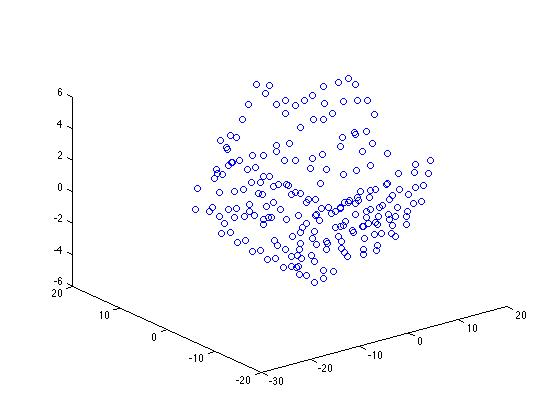
\includegraphics[scale=0.35]{images/house1.jpg}
}
\center
\subfloat[]{
\label{amb}
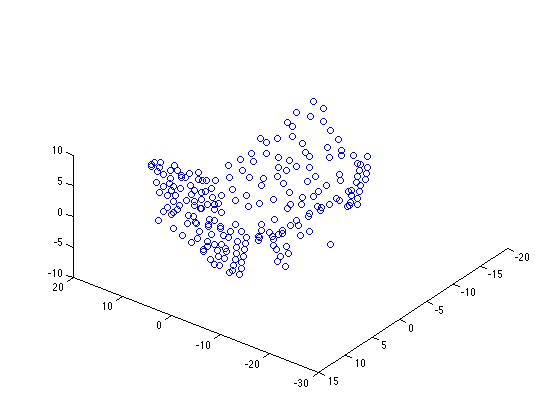
\includegraphics[scale=0.35]{images/house2.jpg}
}
\caption{Reconstruction from house. As can be seen in figure \subref{amb} perpendicular and parallel lines are not preserved.}
\label{rec}
\end{figure}


\subsection{Structure from motion}
We have implemented the Structure from Motion algorithm described in the lecture notes. First we normalize the point coordinates by translating them to the mean of the points in each view. Then, we apply SVD to the measurement matrix, the structure is the matrix $S = W^{\frac{1}{2}} V^T$. The results on the point-view matrix of the house model provided by Rahul Raguram can be found in figure \ref{rec}.

\subsubsection{Point-tracking}
By using our point-tracking algorithm we do not find enough points to recover the structure. The average number of frames that a point is found in is only five frames. We could improve our point-tracking algorithm by using dense SIFT in order to obtain more points that can be matched across the images. However, a consequence of using dense SIFT is that it is computationally more expensive than using just detected interested points and their descriptors. Another option would be to have more frames describing the same motion so that points are visible in more frames.

\subsubsection{Does the reconstruction have an ambiguity?} 
Yes, the reconstruction suffers from affine ambiguity. When rotating the reconstruction so that the actual perpendicular and parallel lines look perpendicular and parallel we can recognize the house clearly. However, this only happens at a specific viewpoint, when viewing the reconstruction differently it is clear that lines that are parallel and lines that are perpendicular have not been reconstructed that way (this can be seen in image \ref{amb}). \subsection{Building 3D model}

\end{document}